\documentclass[9pt,notes]{beamer}
%\documentclass{foils} %if wish to emulate the foils class using beamer

% - Style is ornate.

\mode<presentation>
{
%  \setbeamertemplate{background canvas}[vertical
%shading][bottom=red!10,top=blue!10]

    %% various themes available from the official Beamer user guide
    %\usetheme{default} %% blue, black, and white
    \usetheme{Madrid} %% red, white, and black
    %\usetheme{Frankfurt}
    \usefonttheme[onlysmall]{structurebold}
    %\usefonttheme[onlysmall]{structuresmallcapsserif}

    \setbeamercovered{transparent}
    % or whatever (possibly just delete it)
    %\usecolortheme{beetle}
}

\usepackage{multimedia}
\usepackage[english]{babel}
\usepackage{amsfonts, amsmath, mathrsfs, mathtools}
\usepackage{amsxtra, amsthm, amssymb, amscd}
\usepackage{float}
\usepackage{graphics}
\usepackage{graphicx}
\usepackage{bm}
%\usepackage{subcaption}
\usepackage{latexsym}
\usepackage{multimedia}
\usepackage{hyperref}
\usepackage{xspace}
\usepackage{subfig}
%\usepackage[dvips]{color} \usepackage{color}
%\usepackage{epsfig}
%\usepackage{mathrsfs}
%\usepackage{rotating}
%\usepackage{wrapfig}
%\usepackage[all]{xy}
%\usepackage{verbatim}

\setbeamercovered{dynamic}

\DeclareMathOperator*{\argmin}{arg\,min}
\DeclareMathOperator*{\argmax}{arg\,max}
\DeclareMathOperator{\Exp}{Exp}
\DeclareMathOperator{\grad}{grad}
\DeclareMathOperator{\Log}{Log}
\DeclareMathOperator*{\Cor}{Cor}
\DeclareMathOperator*{\diag}{diag}
\DeclareMathOperator*{\rank}{rank}
\DeclareMathOperator{\tr}{trace}


%%%% color-stuff, e.g., \Green{stuff you want to be printed in green}
\definecolor{LightGray}{rgb}{0.94,0.94,0.94}
\definecolor{VeryLightBlue}{rgb}{0.9,0.9,1}
\definecolor{LightBlue}{rgb}{0.8,0.8,1}
\definecolor{DarkBlue}{rgb}{0,0,0.6}
\definecolor{LightGreen}{rgb}{0.88,1,0.88}
\definecolor{MidGreen}{rgb}{0.6,1,0.6}
\definecolor{DarkGreen}{rgb}{0,0.6,0}
\definecolor{VeryLightYellow}{rgb}{1,1,0.9}
\definecolor{LightYellow}{rgb}{1,1,0.6}
\definecolor{MidYellow}{rgb}{1,1,0.5}
\definecolor{VeryLightRed}{rgb}{1,0.9,0.9}
\definecolor{LightRed}{rgb}{1,0.8,0.8}
\definecolor{Red}{rgb}{1,.2,.1}
\definecolor{Green}{rgb}{0,1,.15}
\definecolor{Blue}{rgb}{.1,.2,1}
\definecolor{Gray}{rgb}{0.5,0.5,0.5}
\definecolor{Black}{rgb}{0,0,0}
\definecolor{White}{rgb}{1,1,1}
\newcommand{\White}[1]{{\color{White}{#1}}}
\newcommand{\VeryLightBlue}[1]{{\color{VeryLightBlue}{#1}}}
\newcommand{\LightBlue}[1]{{\color{LightBlue}{#1}}}
\newcommand{\DarkBlue}[1]{{\color{DarkBlue}{#1}}}
\newcommand{\DarkGreen}[1]{{\color{DarkGreen}{#1}}}
\newcommand{\VeryLightRed}[1]{{\color{VeryLightRed}{#1}}}
\newcommand{\LightRed}[1]{{\color{LightRed}{#1}}}
\newcommand{\Red}[1]{{\color{Red}{#1}}}
\newcommand{\Gray}[1]{{\color{Gray}{#1}}}
\newcommand{\Black}[1]{{\color{Black}{#1}}}
\newcommand{\Blue}[1]{{\color{Blue}{#1}}}
\newcommand{\Green}[1]{{\color{Green}{#1}}}
\newcommand{\LightGray}[1]{{\color{LightGray}{#1}}}

\newcommand{\SELF}[1]{{\note[item]{\Blue{{#1}}}}}
\newcommand{\TODO}[1]{{\note[item]{\Red{{#1}}}}}
\newcommand{\NOTE}[1]{{\note[item]{#1}}}

\newcommand{\R}{\mathbb{R}} % the standard 'set of all real numbers'
\newcommand{\N}{\mathbb{N}} % set of all natural numbers
\newcommand{\Z}{\mathbb{Z}} % integers
\newcommand{\Zpos}{\mathbb{Z}_{+}}
\newcommand{\image}{\mathrm{image}} % image of a function
\newcommand{\spn}{\mathrm{span}}
%
\newcommand{\Vmax}{\ensuremath{\mathcal{V}_{\max}}\xspace}
\newcommand{\Vargmax}{\ensuremath{\mathcal{V}_{\mathrm{argmax}}}\xspace}
\newcommand{\VSigma}{\ensuremath{\mathcal{V}_{\Sigma}}\xspace}
\newcommand{\Vsigma}{\ensuremath{\mathcal{V}_{\sigma}}\xspace}
\newcommand{\Sigmaneg}{\Sigma^{(-)}}	
%
\newcommand{\VSigmapos}{\ensuremath{\mathcal{V}_{\Sigma}^{(+)}}\xspace}
\newcommand{\VSigmaneg}{\ensuremath{\mathcal{V}_{\Sigma}^{(-)}}\xspace}
%
\newcommand{\Vmaxpos}{\ensuremath{\mathcal{V}^{(+)}_{\max}}\xspace}
\newcommand{\Vmaxneg}{\ensuremath{\mathcal{V}^{(-)}_{\max}}\xspace}
\newcommand{\alphapos}{\alpha^{(+)}}
\newcommand{\alphaneg}{\alpha^{(-)}}
\newcommand{\alphaiso}{\alpha_{{\tiny\textsc{ISO}}}}
%
%
\newcommand{\Hess}{\mathrm{Hess}} % fancy H for the hessian
\newcommand{\wein}{\mathsf{L}} % for the Weingarten map
\newcommand{\weinmat}{\widehat{\mathsf{L}}}
\newcommand{\img}{\mathtt{I}} % discrete image (a matrix, not the math term)

\newcommand{\META}{\Red{\textbf{META}}}

\newcommand{\TN}{\mathsf{TN}}
\newcommand{\TP}{\mathsf{TP}}
\newcommand{\FN}{\mathsf{FN}}
\newcommand{\FP}{\mathsf{FP}}

%\DeclarePairedDelimiterX{\inner}[2]{\langle}{\rangle}{#1, #2}
%\DeclarePairedDelimiterX{\vnorm}[1]{\Vert}{\Vert}{#1}
%\DeclarePairedDelimiterX{\abs}[1]{\vert}{\vert}{#1}
%
%\newcommand{\bigO}{\mathcal{O}}
%
%\DeclareMathOperator{\FT}{\mathcal{F}} % fancy F for \FT
%\DeclareMathOperator{\DFT}{\mathcal{D}} % fancy D for \DFT

%%% theorem styles %%%%%%%%%
%\theoremstyle{plain}% default \newtheorem{thm}{Theorem}[section]
%\newtheorem{lem}{Lemma}[section]

%\theoremstyle{definition}
%\newtheorem{defn}{Definition}[section] \newtheorem{exmp}{Example}[section]
%\newtheorem{prop}{Proposition}[section] \newtheorem{cor}{Corollary}[section]

%\newtheorem{property}{Property}[section] \newtheorem{algorithm}{Algorithm}[section]

%\restylefloat{figure} \restylefloat{table}

%\usepackage[latin1]{inputenc} or whatever

\usepackage[T1]{fontenc}
\usepackage{helvet} 
% Or whatever. Note that the encoding and the font should match. If T1
% does not look nice, try deleting the line with the fontenc.

\beamertemplatenavigationsymbolsempty

\title[Cake Defense]{Optimized Strict Multiscale Frangi Prefiltering for Segmentation}
\subtitle{Towards an automated PCSVN extraction}

\author[{Luke Wukmer}] % (optional, use only with lots of authors)
{{Luke Wukmer}}%\inst{1}} \and S.~Another\inst{2}}
% - Use the \inst{?} command only if the authors have different
%   affiliation.

\institute[CSULB] % (optional, but mostly needed)
{
  %\inst{1}%
  Advisor: Dr. Jen-Mei Chang\\
  Department of Mathematics and Statistics\\
  California State University, Long Beach\\
  \texttt{lwukmer@gmail.com}
}
\graphicspath{{./figures/abstract_defense/}
              {./figures/abstract_defense/A-raw_targets/}
              {./figures/}
              {./figures/frangi3d/}
              {./figures/strict_examples/}
              {./figures/inset_of_sample_issues/}
              {./figures/rw_demo/}
              {./figures/output_examples/}
              {./figures/qthresh_demo/}
              {./figures/segmentation_montage/}
              {./figures/segmentation/}
              {./figures/compare_parameters_demo/}
}
\date{April 9, 2019}

\titlegraphic{\includegraphics[height=2cm]{csulb-seal.png}}
\begin{document}

%%% TITLE SLIDE %%%%
\begin{frame} % % % % % % % % % % % % % % % % % % %
  \titlepage
\end{frame}

\section{Introduction}
\begin{frame} % % % % % % % % % % % % % % % % % % % % % % % % %
	\frametitle{Research Goals}
	\begin{columns}[c]
		\begin{column}{0.5\textwidth}
			\begin{figure}
			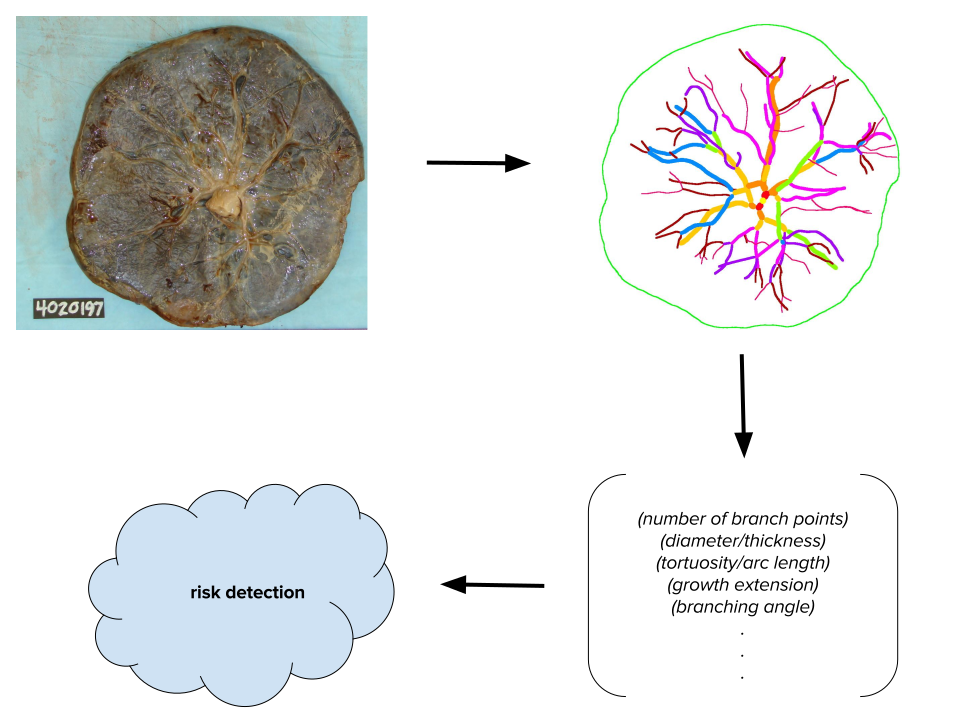
\includegraphics[width=\textwidth]{general_research_question.png}
			\note[item]{In the figure, a manual trace of the placental chorionic
            vascular surface network (PCSVN) is performed.
            This trace is measured in multiple ways. Those measurements are turned into
            a feature vector, which can be used to predict a risk. Refer to Boruta paper.}
			\end{figure}
		\end{column}
		\begin{column}{0.5\textwidth}
			\begin{block}{Vascular Network Extraction in Placentas}
				\begin{itemize}
					\item \textbf{Motivation:}
            Accurate measurement of the vascular structure of a placental sample
            can be used to predict neonatal risk factors, specifically ASD.
					\item \textbf{Challenge:}
						Currently no automated method of obtaining traces of
            PCSVN. Manual tracing is labor intensive but necessary
            for feature analysis.
            \note[item]{Manual tracing requires like 5 hours or something
                  and requires training.
                  There is some guesswork that's done in it too and some limitations
                  in the ground truth itself (will cover later)
                }
					\item \textbf{Research Goal:} Provide a fully automated method of extraction.
          \end{itemize}
			\end{block}
		\end{column}
	\end{columns}
\end{frame}

\begin{frame}
  \frametitle{The Image Processing Problem}
  \begin{columns}[c]
  \begin{column}{0.5\textwidth}
    \begin{itemize}
        \begin{block}{Our image domain}
        \item The PCSVN is a connected network of veins and arteries
                on the surface of the placenta
        \item Ground truth for 201 samples from private NCS dataset
        \item Placentas have been formalin-fixed,
                so arteries are more prominent.
        \item Pictures taken from top down, some glare,
                some inconsistencies.
        \item Placental images are comparatively noisy
        \note[item]{The surface of the placenta has a lot of changes
              in color/topology apart from the PCSVN
              so a lot of techniques that work elsewhere
              for vascular segmentation seem to fail here.
              Thus segmentation is more complicated that than say,
              an eyeball MRI (like original Frangi paper)
            }
      \end{block}
    \begin{block}{Strategy}
      Given the curvilinear nature of these vessels, we will appeal
      to differential geometry.
      \end{block}
    \end{itemize}
  \end{column}
  \begin{column}{0.5\textwidth}
    \centering
    \includegraphics[height=0.48\textheight]{{{T-BN0164923.raw}}} \\[0em]
    %{\Huge $\Downarrow$}\\[-1em]
    \includegraphics[height=0.48\textheight]{{{T-BN0164923.ctrace}}}
    \note[item]{Mention colors are simply vessel widths (3 to 19 odds)
          are part of the tracing protocol. that's really outside of the
          scope of this thesis, but kept anytime we show a ground truth
          because they're pretty
        }
    \note[item]{\META: fix/align/crop the images better}
  \end{column}
  \end{columns}
\end{frame}

%SLIDE 2/12 % % % % % % % % % % % % % % % % % % % % % % % % % % % % % % % % % % % % % % % %
%\begin{frame}
%	\frametitle{Previous Research}
%	
%	\begin{enumerate}[\bfseries(a)]
%	\item Nen Huynh used Frangi filtering result (different data set)
%	\item Frangi filtering is followed by morphological filtering (using principal-directions). Agreement with ground truth is displayed. 
%  \item There's a different research group using a cGAN or whatever and it's really good but
%    resource intensive, but whatever maybe just go with that one
%	\end{enumerate}
%	
%	\end{frame}

\section[Math Methods]{Mathematical Methods}
\begin{frame}
\frametitle{Appealing to Differential Geometry}
  Idealize image as a 3D surface (a graph) with $(x,y)$ spatial coordinates and intensity as the height function.
  \note[item]{Point of this slide is show that finding curvilinear surfaces is reasonable}

  \includegraphics[width=0.3\textwidth]{inset_for_3d_surface}
  \includegraphics[width=0.6\textwidth]{inset_as_3d_surface}
  \note[item]{This point is a lot clearer when you show multiple vessel widths.}
  \note[item]{Also way clearer later when you show the surface after Gaussian blur,
  			  not sure if I should put that here and ``lie''/complicate things early on or not.}
  \note[item]{Crop graph, center, etc}
  \note[item]{\META: Really need to review this whole section to talk about bright/dark
    features; make sure it's clear}
\end{frame}

\begin{frame}
\frametitle{Review of Differential Geometry of (Continuous) Surfaces}
\note[item]{``Let's just pretend we're dealing with this as a continuous surface
              for now''}
  \begin{itemize}
    \item (Thm of Meusnier)
          If you look at a point on the surface and fix a tangent vector,
          then all surface curves through that point with that velocity
          will have the same curvature there.
          So the curvature is intrinsic to the surface, call it normal curvature.
    \item Varying the tangent vector,
          we call extremal values of normal curvature the
          \textbf{principal curvatures}.
          The associated tangent vectors are \textbf{principal directions.}
    \item (Thm. of Olinde Rodrigues)
          These principal curvatures/directions are
          the eigenvalues/eigenvectors of
          a particular map called the \textbf{Weingarten map}.
      \note[item]{Weingarten map also called shape operator. Also can just define
                  the second fundamental form and use that matrix
                  (for our purposes)}
      \note[item]{Note that all this is true for \textit{any} kind of surface,
                  but we really just care about graphs.}
      \note[item]{If you want to get into notation, you can do so as far as explicitly
                  showing what the Weingarten map is (requires Gauss map).
                  You probably can avoid showing any setup of Meusnier--
                  defining curves and so on. 
                  }
  \end{itemize}
\end{frame}

\begin{frame}
\frametitle{Relationship Between Hessian and Weingarten Map for Graphs}
    \begin{block}{Weingarten Map for Graphs}
    Given the graph $f: U \to \mathbb{R}^3$ where $(x,y) \mapsto (x, y, h(x,y))$, the matrix
    representation of its Weingarten map is given by
    \begin{equation*}
    \widehat{\mathsf{L}} = \mathrm{Hess}(h) \tilde{G}
    \end{equation*}
    where
    $
    \tilde{G} := \frac{1}{\left({1+h_x^2 + h_y^2}\right)^{3/2}}   
    \begin{bmatrix}
    1+h_y^2 & -h_x h_y \\
    -h_x h_y & 1 + h_x^2 \\
    \end{bmatrix}
    \;\text{and}\; \Hess(h) = \begin{bmatrix} h_{xx} & h_{xy} \\ h_{yx} & h_{yy} \end{bmatrix}
    $
  \end{block}
  \note[item]{Make sure you have the graph definition clearly here. It's at the top but make it more prominent / earlier slidewise }
  \note[item]{Make point about when we're not at a critical point, we don't guarantee
              any of this (but it seems to work out okay)}
  \begin{block}{Approximating}
    \begin{itemize}
    \item In particular, given a point where $h_x \approx h_y \approx 0$, we
      have $\tilde{G} \approx \mathrm{Id}$, and thus
      $\widehat{\mathsf{L}} \approx \mathrm{Hess}(h)$.
    \item For ease of use, we can simply find eigenvalues of the Hessian instead.
    \note[item]{``Remember this point right here, we will come back to this.''}
    \item This gives rise to a class of filters, the so-called Hessian-based filters.
    \end{itemize}
  \end{block}
\end{frame}

\begin{frame}
  \frametitle{Example: Finding Weingarten map and Principal Curvatures}

\begin{columns}
  \begin{column}{0.5\textwidth}
    \begin{block}{Cylindrical Ridge of radius $r$}
    Let $f$ be the graph given by 
    \begin{gather*}
    f: \R^2 \to \R^3 \;\textrm{by}\; f(x,y) = (x,y,h(x,y)), \\
    \textrm{with}\;
    h(x,y) = \begin{cases}
    \sqrt{r^2 - x^2} & -r < x < r \\
    0 & \textrm{else}
    \end{cases}
    \end{gather*}
  \end{block}
  \end{column}

\begin{column}{0.5\textwidth}
  \includegraphics[width=\linewidth]{circular_trough_with_axes}
\end{column}
\end{columns}

% note: you had these for calculating the gauss map. since you don't need that, just switch to $h$
%\begin{gather*}
%\frac{\partial f}{\partial x} = \left(1, 0, \frac{-x}{\sqrt{r^2 - x^2}}\right)
%\quad , \quad
%\frac{\partial^2 f}{\partial x^2} = \left(0, 0, \frac{-r^2}{\left(\sqrt{r^2 - x^2}\right)^3}\right) \\
%\frac{\partial f}{\partial y} = \left(0, 1, 0\right)
%\quad , \quad
%\frac{\partial^2 f}{\partial y^2} = \frac{\partial^2 f}{\partial x \partial y} = 0
%\end{gather*}

\begin{gather*}
h_x = \frac{-x}{\sqrt{r^2 - x^2}}
\quad , \quad
h_{xx} = \frac{-r^2}{\left(r^2 - x^2\right)^{3/2}}\\
h_y = 0
\quad , \quad
h_{yy} = 0 \quad,\quad h_{xy} = 0
\end{gather*}
\note[item]{Show the example here. Your example calculates from a different definition, like with Gauss map etc. so maybe rework or decide what you want here.}
\note[item]{``Calculate boring partial derivatives''}
\note[item]{Note: the formula for weinmat is on the next slide}
\end{frame}

\begin{frame}
\frametitle{Example: Finding Weingarten map and Principal Curvatures}
\begin{block}{Weingarten matrix representation (for graphs)}
\begin{equation*}
\weinmat = \Hess(h) \tilde{G} \;,\quad \mathrm{where} \quad
\tilde{G} := \frac{1}{\left({1+h_x^2 + h_y^2}\right)^{3/2}}
\begin{bmatrix}
1 + h_y^2 & -h_x h_y \\
-h_x h_y & 1 + h_x^2 \\
\end{bmatrix} 
\end{equation*}
\end{block}

\begin{equation*}
\Hess (h)
  = \begin{bmatrix} h_{xx} & h_{xy} \\ h_{xy} & h_{yy} \end{bmatrix}
   = \begin{bmatrix} \frac{-r^2}{\left(r^2 - x^2\right)^{3/2}} & 0 \\ 0 & 0 \end{bmatrix}
\qquad
\tilde{G} =
  \frac{1}{\left(1+\frac{x^2}{r^2-x^2}\right)^{3/2}}
  \begin{bmatrix}
  1 & 0 \\ 0 & 1 + \frac{x^2}{r^2 - x^2}
  \end{bmatrix}
  \end{equation*}
  \begin{align*}
  \weinmat = \Hess(h)\tilde{G}
           &= \frac{1}{\left(1+\frac{x^2}{r^2-x^2}\right)^{3/2}}
              \begin{bmatrix} \frac{r^2}{\left(r^2 - x^2\right)^{3/2}} & 0 \\
              0 & 0 \end{bmatrix} \\
%           \\
%           &= \frac{1}{\left(\frac{r^2}{r^2-x^2}\right)^{3/2}}
%           \begin{bmatrix} \frac{r^2}{\left(r^2 - x^2\right)^{3/2}} & 0 \\
%           0 & 0 \end{bmatrix}
%          = \frac{\left(r^2-x^2\right)^{3/2}}{r^3}
%          \begin{bmatrix} \frac{-r^2}{\left(r^2-x^2\right)^{3/2}} & 0 \\ 0 & 0 \end{bmatrix}
%          = \begin{bmatrix} \frac{-1}{r} & 0 \\ 0 & 0 \end{bmatrix}
           &= \quad \cdots \quad = \begin{bmatrix} \frac{-1}{r} & 0 \\ 0 & 0 \end{bmatrix}
\end{align*}
\note[item]{This is just some matrix multiplication, exponent rules, and finding common denominators. This would be a good challenge problem for Math 112A minus the matrix.}
\note{ Here's the steps without dots just in case you need to add it back in:
  \begin{align*}
    \weinmat &= \Hess(h)\tilde{G}
  = \frac{1}{\left(1+\frac{x^2}{r^2-x^2}\right)^{3/2}}
  \begin{bmatrix} \frac{r^2}{\left(r^2 - x^2\right)^{3/2}} & 0 \\
    0 & 0 \end{bmatrix} \\
  &= \frac{1}{\left(\frac{r^2}{r^2-x^2}\right)^{3/2}}
  \begin{bmatrix} \frac{r^2}{\left(r^2 - x^2\right)^{3/2}} & 0 \\
    0 & 0 \end{bmatrix}
  = \frac{\left(r^2-x^2\right)^{3/2}}{r^3}
  \begin{bmatrix} \frac{-r^2}{\left(r^2-x^2\right)^{3/2}} & 0 \\ 0 & 0 \end{bmatrix}
  = \begin{bmatrix} \frac{-1}{r} & 0 \\ 0 & 0 \end{bmatrix}
  \end{align*}
}
\note[item]{Mostly, just point out it's $\begin{bmatrix} a & 0 \\ 0 & 0 \end{bmatrix}$ times
  $\begin{bmatrix} b & 0 \\ 0 & c \end{bmatrix}$}
\end{frame}

\begin{frame}
\frametitle{Example: Finding Weingarten Map and Principal Curvatures}
\begin{columns}
  \begin{column}{0.5\textwidth}
    \begin{block}{Cylindrical Ridge of radius $r$}
      Let $f$ be the graph given by 
      \begin{gather*}
      f: \R^2 \to \R^3 \;\textrm{by}\; f(x,y) = (x,y,h(x,y)), \\
      \textrm{with}\;
      h(x,y) = \begin{cases}
      \sqrt{r^2 - x^2} & -r < x < r \\
      0 & \textrm{else}
      \end{cases}
      \end{gather*}
    \end{block}
  \end{column}
  
  \begin{column}{0.5\textwidth}
    \includegraphics[width=\linewidth]{circular_trough_with_axes}
  \end{column}
\end{columns}
\begin{gather*}
\weinmat = \begin{bmatrix} - \frac{1}{r} & 0 \\ 0 & 0 	\end{bmatrix}
\quad \text{Matrix of Weingarten map}\\
u_2 = (1,0) \;,\; u_1 = (0,1)
  \quad \text{principal directions (eigenvectors of $\weinmat$)}\\
\lambda_2 = \frac{-1}{r} \;,\; \lambda_1 = 0
  \quad \text{principal curvatures (eigenvalues of $\weinmat$)}\\
\end{gather*}
\note[item]{\META: need to show what hessian eigs/eigvecs are and emphasize that at the ridge point it's identical}
\note[item]{\META: also can explain (here or later) if there's a stronger signal at the ridge point
  or if it's literally anywhere on the ridge}
\note[item]{
  This is what to stick in somewhere:
  \begin{equation}
  \Hess (h)
  = \begin{bmatrix} h_{xx} & h_{xy} \\ h_{xy} & h_{yy} \end{bmatrix}
  = \begin{bmatrix} \frac{-r^2}{\left(r^2 - x^2\right)^{3/2}} & 0 \\ 0 & 0 \end{bmatrix}
  \end{equation}
  Note that eigenvalues are still $0$ and the top left element (now a function of $x$),
  eigenvectors are (can be chosen to be) the same throughout, and if $x=0$ (at the crest)
  then $\weinmat = \Hess$ exactly, as expected.
}

\end{frame}
\section{The Frangi filter}

\begin{frame}
\frametitle{The (Uniscale) Frangi Filter}
  \begin{equation*}
  \mathcal{V}(x,y) =
  \begin{cases}
  0 & \text{if} \quad \lambda_2 > 0 \\
  \exp\left(-\frac{A^2}{2\beta^2}\right)
  \left(1 - \exp\left(-\frac{S^2}{2c^2}\right)\right) & \text{otherwise}
  \end{cases}
  \end{equation*}
where
\begin{align*}
  A &:= \left|\lambda_1 / \lambda_2\right| \quad\text{(Anisotropy Measure)} \\
  \text{and} \quad 
  S &:= \sqrt{\lambda_1^2 + \lambda_2^2} \quad\text{(Structureness Measure)}
  \end{align*}

for eigenvalues $\lambda_1, \lambda_2$ of the Hessian (at point (x,y)),
   $ \left|\lambda_1\right| \leq \left|\lambda_2\right|$

and $\beta$ and $c$ are parameters

\note[item]{Mostly point out how it all fits together. Two simple functions of the principal
  curvatures, put into exponential forms, with a parameter to control each.}
\note[item]{``We'll go through this step by step and look at each part more closely''}
\note[item]{Mention that if you wanted to use the ``real'' principal curvatures here you're more than welcome to}
\note[item]{Don't need to spend too much time on this slide, we'll put it back again}
\end{frame}

\begin{frame}
\frametitle[Anisotropy Factor]{Frangi filter anatomy}
\begin{block}{Anisotropy Factor}
\begin{equation}
\exp\left(-\frac{A^2}{2\beta^2}\right) \quad,\quad
A := \left|\frac{\lambda_1}{\lambda_2}\right|
\end{equation}
\end{block}
\begin{itemize}
  \item For selecting anisotropic content (lines not blobs)
  \item When $A$ is very close to 0,
  $\left|\lambda_2\right| \gg \left|\lambda_1\right|$, and the factor is $\approx 1$.
  \item Choosing parameter: Frangi suggested $\beta=\frac{1}{2}$ as a reasonable default.
\end{itemize}
\begin{figure} \centering
  \subfloat[Anisotropic]{
\includegraphics[width=0.5\linewidth]{circular_trough_with_axes}}
\subfloat[Isotropic]{
\includegraphics[width=0.3\linewidth]{hemisphere_wolframalpha}}
\end{figure}
\end{frame}

\begin{frame}
\frametitle[Structureness Factor]{Frangi filter anatomy}
\begin{block}{Structureness Factor}
  \begin{equation}
  \left(1 - \exp\left(-\frac{S^2}{2c^2}\right)\right)
  \quad,\quad
  S := \sqrt{\lambda_1^2 + \lambda_2^2}
  \end{equation}
\end{block}

\begin{itemize}
  \item This selects content with significant curvature.
  \item Purpose is to filter out numerically small values, we only want significant curvilinear content ($S$ large).
  \note[item]{For example, we don't want our filter to report a point as curvilinear structure if $\lambda_1 / \lambda_2$ is large, but we can't differentiate between
  $\lambda_2 = 100, \lambda_1 = .01$ and $\lambda_2 = .001, \lambda_1 = .000001$}
  \item Important to pick a reasonable value for the image at hand / image domain.
  \note[item]{This is actually critically important to define, entire filter will be
              extremely noisy otherwise. Less important in MRI images, but more important
              for our context where there is significant noise. Talk about the standard implementation where c=15 is the default for seemingly no reason.}
  \item Frangi suggested ``half the maximum value of the Hessian norm''. We will define
  the parameter $\gamma$ and define $c(\gamma) = \gamma S_{\max}$, since $S_{\max}$ is the
  Frobenius norm of the Hessian.
\end{itemize}
  \note[item]{I'm not sure when/how to introduce $\gamma$ instead but it should be
  prominent enough that I don't have to worry about using it exclusively
  in later slides}
\end{frame}

\begin{frame}
\frametitle{Frangi filter anatomy: Putting it together}
\begin{block}{Frangi filter}
 \begin{equation}
\Vsigma(x_0,y_0) =
\begin{cases}
0 & \text{if} \quad \lambda_2 > 0 \\
\exp\left(-\frac{A^2}{2\beta^2}\right)
\left(1 - \exp\left(-\frac{S^2}{2{(\gamma S_{\max})}^2}\right)\right) & \textrm{otherwise}
\end{cases}
\end{equation}
\begin{equation}
\textrm{where} \quad A := \left|\lambda_1 / \lambda_2\right|
\quad \textrm{and} \quad 
S := \sqrt{\lambda_1^2 + \lambda_2^2}
\quad, \left|\lambda_2\right| \ge \left|\lambda_1\right|
\end{equation}
\end{block}
\begin{itemize}
\item $\lambda_2 > 0$ means the point would be a local minimum (at a critical point). We are looking for a local maximum by looking for bright curvilinear objects. You can switch this ($\lambda_2 < 0$ as the case) if you are looking for dark curvilinear.
\item Point of $\exp(...)$ and $1 - \exp(...)$ structure is that the filter decays rapidly as anisotropy or structureness decrease.
\end{itemize}
\note[item]{\META: Really look into the bright/dark curvilinear subject and try to explain better.}
\note[item]{\META: Significance of sign of principal curvature (real one from Weingarten map)?}
\note[item]{\META: Get rid of the sigma until after scale space theory?}
\note[item]{If it's too long to get to this point, maybe start showing samples already}
\end{frame}
\begin{frame}
\frametitle[Frangi parameters]{Frangi filter anatomy: Choosing Parameters}
%\begin{block}{Frangi filter}
  \begin{equation}
  \Vsigma(x_0,y_0) =
  \begin{cases}
  0 & \text{if} \quad \lambda_2 > 0 \\
  \exp\left(-\frac{A^2}{2\beta^2}\right)
  \left(1 - \exp\left(-\frac{S^2}{2{(\gamma S_{\max})}^2}\right)\right) & \textrm{otherwise}
  \end{cases}
  \end{equation}
  \begin{equation}
  \textrm{where} \quad A := \left|\lambda_1 / \lambda_2\right|
  \quad \textrm{and} \quad 
  S := \sqrt{\lambda_1^2 + \lambda_2^2}
  \quad, \left|\lambda_2\right| \ge \left|\lambda_1\right|
  \end{equation}
%\end{block}
\includegraphics[width=0.49\textwidth]{4} % beta=0.1 gamma=1.0
\includegraphics[width=0.49\textwidth]{14} % beta=0.5 gamma=0.5 
\begin{itemize}
\item We will show a lot of data with different choices of parameters later.
\end{itemize}
\end{frame}

\begin{frame}
\frametitle[Scale Space Theory]{Linear Scale Space Theory for Kids}
\begin{itemize}
  \item Obviously the image is not actually a continuous surface.
        It is a particular sampling of a surface. 
  \item We want to embed the image this image with a ``resolution'' parameter.
  \item Motivate and say some basic axioms.
  \item Convolution by Gaussian solves these problems, discrete derivatives are fine too
\end{itemize}

\begin{block}{Axioms}
  \begin{itemize}
    \item Linear shift and rotational invariance
    \item Semigroup property
    \item Continuity of scale parameter
    \item Causality condition
    \end{itemize}
  \note[item]{Maybe spend an extra slide on causality condition.
              Basically, as resolution decreases (scale increases) then local minima do not
              decrease, and local maxima do not increase.}
  \note[item]{Prepare a couple more details to get into here.}
  \end{block}
\end{frame}

\begin{frame}
\frametitle{Implementation Detail: Calculating Discrete Hessian}
\begin{columns}
  \begin{column}{0.4\textwidth}
    \begin{itemize}
      \item Convolution by gaussian matrix is slow. 
      \item Calculate in frequency space as a multiplication
    \end{itemize}
  \end{column}
\begin{column}{0.6\textwidth}
  \includegraphics[width=\textwidth]{convolution-runtime-demo-alt}
\end{column}
\end{columns}
\TODO{Add some of the math but not too much}
\TODO{Why is this so much faster now?}
\NOTE{This is short. Mention MSE findings}
\end{frame}

\begin{frame}
\frametitle{Frangi Filter Anatomy: Scale parameter}
  \note[item]{Mention general relationship between vessel width.}
  \note[item]{Describe relative strength of outputs and what's too large.}
  \SELF{This is unscaled output}
\includegraphics[width=\textwidth]{scalesweep_stitch_BN5280796_inset}
\begin{center}
\includegraphics[width=0.75\textwidth]{scalesweep_colorbar}
\end{center}
\end{frame}

\begin{frame}
%\frametitle{Frangi Filter Anatomy: Scale parameter}
\note[item]{Same thing but whole plate. Show this for like 5 seconds.}
\note[item]{``This is basically just to show that these trends work throughout the whole image, etc''}
\includegraphics[width=\textwidth]{scalesweep_stitch_BN5280796_plate}
\begin{center}
  \includegraphics[width=0.75\textwidth]{scalesweep_colorbar}
\end{center}
\end{frame}

\begin{frame}
\frametitle{Multiscale Frangi filter}
For a set of scales to probe, $\Sigma := \left\{ \sigma_0, \sigma_1 , \cdots, \sigma_n \right\}$,
the set of $n$ scales at which to probe,
\begin{equation}
\Vmax(x_0, y_0) :=
\underset{\sigma \in \Sigma}{\max}\left\{  \Vsigma (x_0, y_0) \right\}
\end{equation}
where \Vsigma is the Frangi vesselness measure at scale $\sigma$ for the pixel $(x_0,y_0)$

\begin{block}{Notes}
\begin{itemize}
  \item The default ``merging'' strategy suggested by Frangi.
  \item Alternatively, we can process each scale by itself too if we want to.
  \item Decide what scales to use:
    \begin{itemize}
      \item Logarithmic spacing makes some intuitive sense.
      \item Need to experiment to determine what is large / small enough.
      \item Smaller scales for smaller features, larger scales for larger features.
    \end{itemize}
  \note[item]{We can also keep track of $\Vargmax$ etc.}
  \note[item]{Recall that this is a probability-like measure, so this is the probabilityish
              that it has the differential geometry of a curvilinear structure}
\end{itemize}
\end{block}
\end{frame}


\section{Research Protocol}
\begin{frame}
\frametitle{The data set}
\begin{center}
\includegraphics[height=\textheight]{bad_gallery_rot}
\end{center}
\NOTE{Just talk about how some are better than others, some are bad perfusion, some have issues
  with bordering and UCIP point (default methods didn't work well). A few have very nonstandard
  vessel widths.}
\NOTE{We'll look at some of the issues with ground truth in detail in a minute}
\NOTE{Basically, since you've already explained the data set earlier, this is for explaining
  the wide variation in sample quality}
\TODO{Better to have single samples with Frangi outputs to explain how it's not good}
\end{frame}

\begin{frame}
\frametitle{Ground truth}
\begin{figure}[p] \centering
  \subfloat{\includegraphics[width=0.40\textwidth]{{{T-BN0164923.raw}}}
  }
  \subfloat{\includegraphics[width=0.40\textwidth]{{{T-BN0164923_perimeter_overlay}}}
  }\\[-.2cm]
  \subfloat{
    \includegraphics[width=0.40\textwidth]{{{T-BN0164923_arteries_overlay}}}
  }
  \subfloat{
    \includegraphics[width=0.40\textwidth]{{{T-BN0164923_veins_overlay}}}
  }
%  \subfloat{
%    \includegraphics[width=0.35\textwidth]{{{T-BN0164923_all_layers_overlay}}}
%  }
\end{figure}
\note[item]{Maybe show these cropped, who cares}
\note[item]{Maybe show enlarged UCIP and border, IDK if these will show up well}
\note[item]{Maybe show cropped, merged trace by itself on one slide (quickly)}
\end{frame}

\begin{frame}
\frametitle{Imperfections/Complications in Data set}
\begin{figure}
  \includegraphics[width=\textwidth]{annotations-montage-2by2}
\end{figure}
\TODO{The $2\times 2$ annotations might be too complicated, might not show up on the projector. Maybe just switch between two slides? or show different colors of annotations on each slide?}
\NOTE{Talk about:
  \begin{itemize}
    \item UCIP noise
    \item too small and too big
    \item bad perfusion
    \item crossings
  \end{itemize}}
\end{frame}

\begin{frame}
\frametitle{Preprocessing: Dealing with Glare}
\begin{center}
\includegraphics[height=0.8\textheight]{glare_inset_demo_labeled_zealous}
\end{center}
\NOTE{Glare isn't catastrophic in most cases, but it can throw off results.}
\NOTE{We're looking for small abrupt peaks on the surface, want to smooth out.}
\NOTE{For simplicity, we assume everything higher than $175/255$ is glare}
\NOTE{MATLAB has a technique called imfill that solves Laplace equation $\nabla f = 0$.
  We use built-in python that does biharmonic equation $\nabla\nabla f = 0$. It's pretty slow,
  so we speed it up by using an alternate strategy, where we just take the median of the boundary
  for smaller masked regions. You can see the lowest portion of the middle mask is fixed in the
  hybrid method.}
\SELF{Times to process a representative sample (whole thing not this inset):
  \begin{itemize}
    \item biharmonic inpainting: 22 seconds
    \item boundary median 4 seconds
    \item hybrid method 6 seconds
  \end{itemize}
}
\TODO{Would be nice to have implementation details on the slide but I'm worried you can't }
\end{frame}

\begin{frame}
\frametitle{Preprocessing: Umbilical Stump}
\begin{center}
\includegraphics[height=0.9\textheight]{ucip_demo}
\end{center}
\NOTE{It was hard to remove these in an automated way that worked for all samples. You could do a white top hat and have it work a good amount of the time, but I ran out of time to do it effectively. There isn't any good data here due to diffgeo anyway as far as I can tell. Tracing protocol seems to estimate a lot.}
\SELF{This was with a radius of 50 pixels}
\NOTE{This prevents area around the stump from being misconstrued as part of vascular network.}
\SELF{Basically picked this particular one because you can see that the radius we picked doesn't exactly fix the issue, but it does make it better. Hard to tell that the signal is \textit{too} much better, but we see (also from the lack of reporting these as false positives) a minor improvement in precision and MCC scores throughout.}
\TODO{Zoom in would be nicer if you have time}
\end{frame}

\begin{frame}
\frametitle{Preprocessing: Dealing with Boundaries}
\begin{center}
\includegraphics[height=0.8\textheight]{boundary_dilation_demo_labels}
\end{center}
\NOTE{Prevent curvilinear content around the edges from being interpreted as curivilinear (especially with bounding structureness).}
\note[item]{This can be especially significant with certain choices of dark/light BG and at small or large scales. Doesn't matter sooooo much, it's more of a quality of life thing.}
\note[item]{Mostly because we want the background to be ignored, not treated as minimum (or maximum) intensity.}
\note[item]{Since we already know where the mask is, we can just dilate it by a fixed amount (this is by 25 pixel radius)}.
\TODO{Urgent: You need to describe watershedding procedure}
\NOTE{Note the different response for light features when the border is removed}
\end{frame}

\section{Analysis (Pre-segmentation)}

\begin{frame}
  \frametitle{Comparing Frangi Hessian to Frangi with Weingarten Map}
  \begin{figure}[p]\centering
    \subfloat[Raw Sample]{
      \includegraphics[width=0.32\textwidth]{BN4384182-raw-weindemo}
  }
    \subfloat[$\mathcal{V}_{\max}$ (Hessian eigvals)]{
      \includegraphics[width=0.32\textwidth]{BN4384182-Vmax-weindemo}
  }
    \subfloat[$\mathcal{V}_{\max}$ (Weingarten eigvals)]{
      \includegraphics[width=0.32\textwidth]{BN4384182-Wmax-weindemo}
  }
  \end{figure}
\begin{itemize}
  \item Finding Hessian eigenvalues is about 16 times faster
        (25 scales 24 seconds vs. 7 minutes. mean of 25 samples)
  \note[item]{Hessian matrix is much easier to find eigenvalues of}
  \item Scale dependency not the same
  \note[item]{Admit that this came pretty late into my research adventure so I need to look at this more. Weingarten map gives valid response at higher scales than the Hessian. Better
    at outlining just the ridge. Would like to compare strict Frangi to just Weingarten map}
  \item Frangi parameters seem less important for Weingarten map
  \note[item]{Note, noise is noise; still present.}
  \note[item]{You could potentially do a hybrid, i.e.
  recalculate significant Frangi responses like this. Also there could be a speedup by not doing \textit{every} non-masked point, i.e. make sure that hessian magnitude is large enough first. that would be fast.}
  \TODO{Move to late in talk, otherwise rest of this shit kinda feels weak.}
  \TODO{Also, need to look at
    \texttt{skimage.feature.hessian\_matrix\_eigvals}
    to figure out other reasons for speedup/ask von Brecht}
  \SELF{Scales are kinda wrong for optimal Hessian-Frangi, hence more noise there}
\end{itemize}
\end{frame}

\begin{frame}
\frametitle{Cumulative Vesselness Ratio}
\begin{columns}
  \begin{column}{0.6\textwidth}
    \begin{center}
    \includegraphics[height=0.9\textheight]{BN6028328-3x3params-190322}
    \end{center}
  \end{column}
  \begin{column}{0.4\textwidth}
    \begin{table}[p]\centering
      \begin{tabular}{|c|c|c|}
        \hline
        \textbf{label}  & $\bm{\beta}$ & $\bm{\gamma}$ \\ \hline
        standard & $0.5$ & $0.5$ \\ \hline
        loose & $ 1.0$ & $0.3$ \\ \hline
        strict & $0.10$ & $1.0$ \\ \hline
        semiloose-$\beta$ &$ 1.0$ & $0.5$ \\ \hline
        semistrict-$\beta$& $ 0.1$ &$ 0.5$ \\ \hline
        semiloose-$\gamma$ &$ 0.5$ & $0.3$ \\ \hline
        semistrict-$\gamma$& $ 0.5$ & $1.0$ \\ \hline
        anisotropy only & $ 0.5$& $0$ \\ \hline
        structureness only&  $ \infty$ & $0.5$ \\ \hline
      \end{tabular}
    \end{table}
  \end{column}
\end{columns}
\end{frame}

\begin{frame}
\includegraphics[width=\textwidth]{cvr_boxplot_wide-all-ucip-190322}
\end{frame}

\section{Frangi Segmentation Methods}

\begin{frame}
\frametitle{Fixed threshold of Vmax}
\end{frame}

\begin{frame}
\frametitle{Scalewise percentile filtering}
\end{frame}

\begin{frame}
\frametitle{Signed Frangi}

\end{frame}

\begin{frame}
\frametitle{Signed Frangi}
\includegraphics[width=\textwidth]{signsweep_stitch_BN5280796_inset_alt}
\begin{center}
  \includegraphics[width=0.75\textwidth]{signsweep_colorbar_alt}
\end{center}
\end{frame}

\begin{frame}
\frametitle{A non-Frangi segmentation method: ISODATA}
This represents a good idea that doesn't rely on diffgeo or local anything
\TODO{Find histogram figure}
\TODO{Put an output here}
\end{frame}

\section{Frangi Segmentation Results}
\begin{frame}
\frametitle{Binary Classification of Segmentation Methods}
\begin{columns}
\begin{column}{0.4\textwidth}
\begin{figure}
  \centering
  \includegraphics[height=0.5\textheight]{example_confusion_small} \\
  \includegraphics[height=0.2\textheight]{confusion_legend}
\end{figure}
\end{column}
\note[item]{\META: Use GIMP to merge legend with image and put horizontal under image. maybe add precision and mcc of this particular example}
\begin{column}{0.6\textwidth}
  \begin{block}{Scoring Methods}
  \begin{equation*}
  \textsf{precision} \;=\; \frac{\TP}{\TP+\FP}
\end{equation*}

\begin{equation*}
\textsf{MCC} = \frac{\TP\times \TN - \FP \times \FN}{\sqrt{ (\TP+\FP)(\TP+\FN)(\TN+\FP)(\TN+\FN)}}
\end{equation*}
\note[item]{There are a lot of different choices in terms of scoring, like accuracy (list more)}
\note[item]{Rationale behind MCC, the benefit}
\note[item]{Explain that MCC is good but precision is important too}
\note[item]{Would be good to have a scoring method based on network, but that's definitely nontrivial to define}
\end{block}
  \end{column}
\end{columns}
\end{frame}

\begin{frame}
\frametitle{Example Segmentation Results}
Spend a couple slides here talking about
\begin{itemize}
  \item parametrization choices effect
  \item threshold choices effect
  \item talk about ``good'' false positives and  ``bad'' false positives
  \item talk about good samples and bad samples
\end{itemize}
\end{frame}

\begin{frame}
\frametitle{Boxplots}
\begin{center}
\includegraphics[height=0.8\textheight]{190408-all-MCC-boxplot-semistrict}
\end{center}
\end{frame}

\begin{frame}
\frametitle{Boxplots test with both}
\begin{center}
\includegraphics[width=0.48\textwidth]{190408-all-MCC-boxplot-semistrict}
\includegraphics[width=0.48\textwidth]{190408-all-precision-boxplot-semistrict}
\end{center}
\end{frame}

\begin{frame}
\frametitle{Conclusion}
\end{frame}

\appendix
\newcounter{finalframe}
\setcounter{finalframe}{\value{framenumber}}
% Backup frames

\begin{frame}
\frametitle{Appendix}
Put some proofs / extra things here
\end{frame}

\begin{frame}
extra blah blah
\end{frame}
\begin{frame}
another extra slide
\end{frame}
\setcounter{framenumber}{\value{finalframe}}
\end{document}